% 2023本郷祭 マイコン部 部誌 「マイコンHONGOMagazine」 TeXテンプレート

% =環境設定=

\documentclass[b5paper,9pt,platex,dvipdfmx]{jsarticle}

% 数式
\usepackage{amsmath,amsfonts}
\usepackage{bm}

% 画像
\usepackage[dvipdfmx]{graphicx}
\usepackage{float}

% 段組
\usepackage{multicol}
\setlength{\columnseprule}{0.5pt}

% 余白
\usepackage[paper=b5j,truedimen,margin=15truemm,dvipdfmx]{geometry}

% ページ番号を削除
\pagestyle{empty}

% ソースコード環境
\usepackage{listings,jlisting}
\lstset{
  basicstyle={\scriptsize\ttfamily},
  identifierstyle={\scriptsize},
  commentstyle={\smallitshape},
  keywordstyle={\scriptsize\bfseries},
  ndkeywordstyle={\scriptsize},
  stringstyle={\scriptsize\ttfamily},
  frame={tb},
  breaklines=true,
  columns=[l]{fullflexible},
  numbers=left,
  xrightmargin=0zw,
  xleftmargin=0zw,
  numberstyle={\scriptsize},
  stepnumber=1,
  numbersep=1zw,
  lineskip=0.5ex
}
\renewcommand{\lstlistingname}{リスト}

% 枠付き文字(引用文)
\usepackage{fancybox}
\usepackage{ascmac}

% URL
\usepackage{url}

% 書きたい内容に合わせてお好きなパッケージを導入していただいて構いませんが、外部パッケージは提出時に必ず合わせて提出してください。
% また、そのパッケージを使用している部分には必ずコメントをしてください。

% =環境設定ここまで=

\begin{document}

% =タイトル=
\title{PC-9800完全制覇}
\author{H.Taido}
\date{\today}
\maketitle
% 初めのページのページ番号を削除(\maketitleの影響を回避)
\thispagestyle{empty}

% ここではページごとに段組しています。大きく画像を表示したいときなどは以下を \begin{multicols}{3} 、\end{multicols}のように変更すると文章が終わった直後から空白になります
\begin{multicols*}{3}
  
% 以下本文
\section*{ピポッ!}
皆さんこんにちは。名誉部長\footnote{我が部では中3と高2のみ部長になれるため、高1は部長になれません。ですが周りから部長っぽい仕事をさせられているうちに名誉部長とか呼ばれるようになってしまいました(笑)}のH.Taidoです。\\
今回は、{\bf PC-9800シリーズ 完全制覇}ということで、PC-9800シリーズの大体のことについて説明していきたいと思います。\\共に約30年前にタイムスリップし、当時のPCやそれを取り巻く文化について見ていきましょう。\footnote{おいお前何歳だという質問には、残念ながら応じることができません。(当時を知る方で間違っていることがありましたらこっそり教えて下さい!)}\\
拙文ではありますがよろしくお付き合いください。
\section*{目次}
\begin{itembox}[l]{Index}
  1. 98の概要

  2. 身近な98

  3. 98の何がいいの?

  4. ハードの紹介
  \\〜機種の見分け方を添えて

  5. ソフト
  \\〜OSの変遷とPC文化の変容

  コラム 98の歴史

  6. 今から始めるPC-98
  \\〜ソフト編

  7. 今から始めるPC-98
  \\〜ハード編

  8. おわりに
  \end{itembox}
\part{PC-9800って?}
ではまず手始めにPC-9800シリーズとは何か、から簡単にご説明しましょう。
\section[short]{Wikipedia}
\begin{screen}
PC-9800シリーズは、日本電気(以下NEC、現在はNECパーソナルコンピュータに分社)が1982年(昭和57年)から2003年(平成15年)9月30日の受注終了まで、日本市場向けに販売していた独自アーキテクチャのパーソナルコンピュータ(パソコン)の製品群である。同社の代表的な製品であり、98(キューハチ/キュッパチ)、PC-98などと略称されることもある。
\end{screen}
\rightline{Wikipediaより}\footnote{ウィキペディアの執筆者. “PC-9800シリーズ”. ウィキペディア日本語版. 2023-05-04. \url{https://ja.wikipedia.org/w/index.php?title=PC-9800シリーズ&oldid=95052434}, (参照 2023-08-01).}
\\
\\
はいそうですWikipediaです。
これは別に私が調査不足というわけでも書くのをサボっているというわけでもなく、辞書的な説明をするにはやはり百科事典を引用するのが最適であるという研究の成果なのであります(汗)。
\section[short]{補足}
とはいえ上の説明では「???」な方もいると思われるので少し補足をば。

PC-9800シリーズは、1980年代から2000年代まで販売されていたパーソナルコンピュータ(PC)のシリーズの総称です。全盛期には日本中のパソコンの約9割がこのシリーズでした。50代以上の方には馴染みのある響きがあるのではないでしょうか。

先の文章で、「独自アーキテクチャ」というのが一番わからないポイントだと思います。ここについて深掘りして解説しましょう。
現代のPCでは、違うPC(たとえば、製造会社の違いなど)であっても同じソフトウェアが動くのが一般的でしょう。
実は、これはとても不思議なことなのです。コンピュータという機械はあらゆる部品が複雑に組み合わさってできています。ですから、これを一つ組み換えてしまっただけでも、もうそのコンピュータの作りは他とは別物になってしまいます。そして作りが違うのなら同じ動作はしなくなるはずです。\\
すべてのコンピュータにまったく同じ部品を使っているわけではありませんから、当然違うコンピュータでも同じソフトウェアが動作することには何か理由があるはずです。なぜでしょうか?\\
これは、{\bf 同じ設計図を元にして、各社がそれに当てはまるようにして作っている}からです。\\
どういうことかというと、まず、あるコンピュータがあります。それには設計図が存在します。そして、次のコンピュータを作るときには、その設計図を元にして、改良を加えながらも元の部品と同じ仕組みで動作する\footnote{このことを、「{\bf 互換性を持たせる}」と言います。}ようにするのです。この設計図のことを「{\bf アーキテクチャ}」と呼びます。\\
現代のPCはx86-64アーキテクチャに基づいています\footnote{わかりやすくするため、ISA(CPUの命令セットアーキテクチャ)にのみ触れています。\\また、いわゆる「パソコン」ではx86-64が主流ですが、Appleシリコン製Macやスマートフォンなどのモバイル端末では「ARM64」アーキテクチャが主流です。}。これに沿って各社がコンピュータを作ることで、異なるコンピュータでも同じソフトウェアが動作するのです。\\
さて、PC-9800シリーズの発売された当初は、まだ業界標準となるアーキテクチャが考案されておらず、各社がそれぞれアーキテクチャを考案していました。というわけで、PC-9800シリーズはNECの「独自アーキテクチャ」を採用したコンピュータのシリーズだ、と言えるわけです。

ここまでアーキテクチャについて(補足の域を超えて)かなり詳しく説明しましたが、当然意味もなく説明したわけではありません。この「アーキテクチャの独自性」が、今後のPC-9800シリーズ(特に歴史)について語る上で、非常に大切になってきます。どのような点が重要なのかは...次章からのお楽しみとしましょう。
\part{身近なPC-98}
\setcounter{section}{0}
概要の説明を終えたわけですが、読者の皆様の中には「ふーん、それで?」と思われた方もいらっしゃるかもしれません。ここで、身近なところに関わっているPC-98\footnote{PC-9800シリーズ全般のことを、以後「PC-98」と呼称します。}についてご紹介しましょう。PC-98について少しでも興味を持っていただければ幸いです。
\section[short]{今なお現役}
PC-98はバブル時代にその最盛期を迎えました。その頃作られた工場などではPC-98を設計ソフトや生産ライン管理システムとして導入しているものが数多くあります。。先述の通りPC-98は独自アーキテクチャであるため、最新のPCに更新するためにはその工場の全ての設備やソフトウェアを交換しなければなりませんが、とてもそんな費用は出せない...というとことで、NECによる販売やサポートが終了した今でも、PC-98が現役で稼働している工場などが存在しています。また、これらの現場を支えるためPC-98を修理する業者もあります。
身近なところでは、お台場周辺を走る新交通システム「ゆりかもめ」でも、2020年7月まで(!?)PC-98を設備メンテナンス用途で使用していたそうです。
\section[short]{日本のサブカルチャーに与えた影響}
ところで。皆さんはこんなものを見たことはありますか?
\begin{figure}[H]
  \centering
  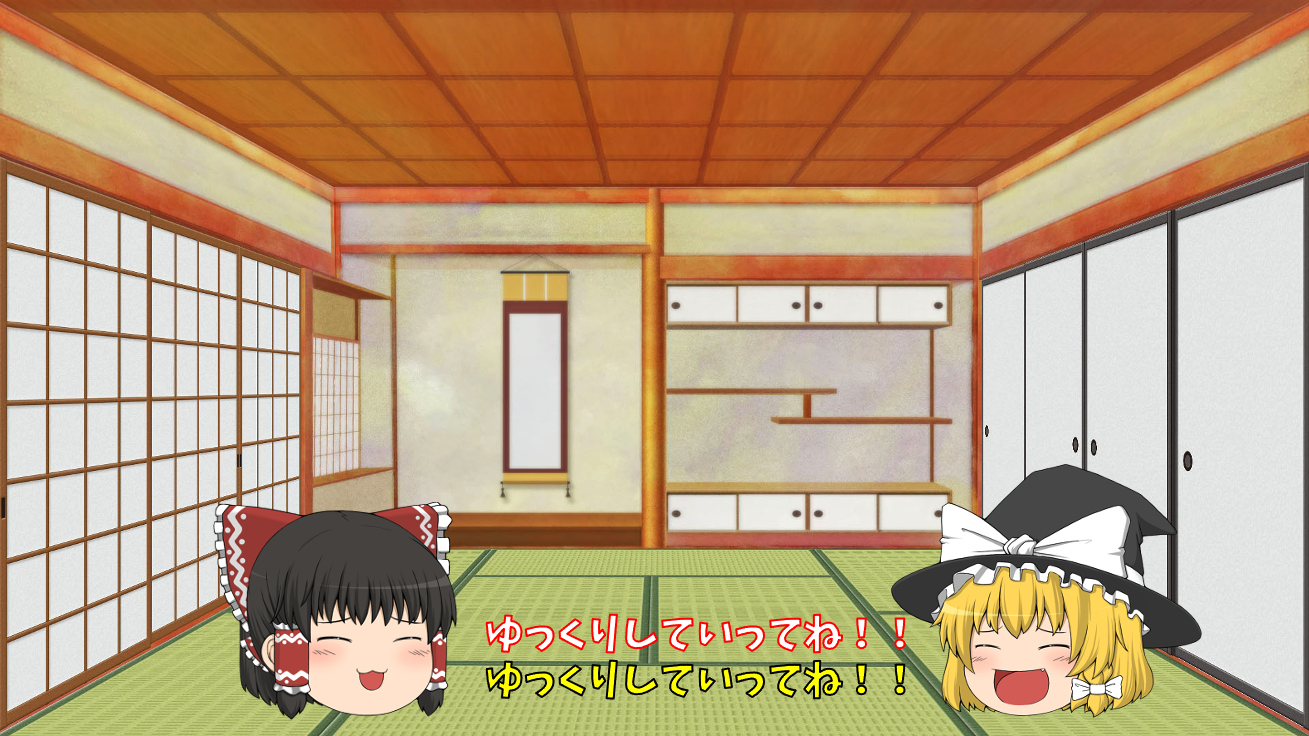
\includegraphics[width=6cm]{img-1.png}
  \caption{ゆっくりしていってね!!!}
\end{figure}
  おそらく一度は見たことがあると思うのですが、こちらは「ゆっくり」と呼ばれる謎の人頭饅頭です。現在、YouTube他多くのインターネット上のプラットフォームのあらゆる界隈に進出しており、「ゆっくり実況」「ゆっくり解説」「ゆっくり茶番劇」などの多彩な動画ジャンルを産んでいます。Googleで、「ゆっくり」のワードで動画検索をかけると、その数は約 35,200,000 件にも及びます。\\
実は、ゆっくりの誕生にもPC-98が深く関わっているのです。

ゆっくりには元ネタがあります。「れいむ」「まりさ」「さなえ」「ようむ」などの名前が何なのか気になって調べた人も中にはいるのではないでしょうか。ゆっくりはゲーム「東方Project」に登場するキャラクターが元になったものなのです。\\
それをインターネット掲示板「2ちゃんねる」(現5ちゃんねる)上の誰かが、人頭饅頭型の霊夢・魔理沙\footnote{どちらも東方Projectのキャラクターの一人です。}が「ゆっくりしていってね!!」と喋っているAA(アスキーアート)を作ったのが始まりです。\\
そしてなんと、元ネタとなったゲーム「東方Project」は、PC-98のゲームなのです。\footnote{東方Project第1弾~第5弾までが、PC-98上で動作するように作られました。}\\
PC-98中期~後期には、それまで企業や一部の物好きな金持ちのものだったコンピュータが、一般家庭にも普及し始めました。その中で、PC-98は東方Projectをはじめとする多くのゲームや音楽などを通して、日本のサブカルチャーの発展に大きな影響を与えたのです。PCとそれに関わる大衆文化について考えるには、PC-98の歴史を知ることが不可欠、と言えるでしょう。
\part{98の何がいいの?}
\setcounter{section}{0}
さて、ここまでの文章を読んですでに読者の皆様は「早くPC-98について教えてくれよ!!!!」と期待絶頂であるかと推察いたしますが、いかがでしょうか(笑)\\

...え?

\begin{screen}
98がすごいPCだということはまあわからんでもない。でも、そんな30年前の骨董品をいじって何が楽しいんだ?」
\end{screen}
...わかりました!!そこまで仰るのなら存分に語って差し上げましょう!!\footnote{このように、ヲタクと呼ばれる人種に不用意にこのような質問をすると長時間拘束されること請け合いですので、ぜひともご注意ください。}
\end{multicols*}
...?
\end{document}